
\documentclass[11pt]{article}
\PassOptionsToPackage{svgnames}{xcolor}
\usepackage{graphicx} % Required for inserting images
\usepackage[utf8]{inputenc}
\usepackage[margin=1in]{geometry}
\usepackage{enumerate, fancyhdr, color, verbatim, setspace, multirow, multicol,subcaption, booktabs, caption, amsfonts}
\usepackage{rotating}
\usepackage{amsmath}
\usepackage{amsthm}
\usepackage{listings}
\numberwithin{equation}{section}

\theoremstyle{definition} 
\newtheorem{definition}{Definition}[subsection]
\newtheorem{theorem}{Theorem}[subsection]
\newtheorem{corollary}{Corollary}[subsection]

\usepackage{colortbl}
\usepackage{tikz}
\usetikzlibrary{matrix, positioning, shadings, shadows}
\usepackage{pgfplots}
\pgfplotsset{compat=1.18}
\usepackage[shortlabels]{enumitem}
% \usepackage[symbol]{footmisc}
\usepackage{multirow}
\usepackage{multicol}
% Creates the header and footer. You can adjust the look and feel of these here.
\usepackage{hyperref}
\hypersetup{
    colorlinks,
    citecolor=black,
    filecolor=black,
    linkcolor=blue,
    urlcolor=blue
}
\newcommand{\bp}{\mathbb{P}}

\definecolor{lightgray}{RGB}{230, 230, 230}
\definecolor{lightgrey}{RGB}{200, 200, 200}

\usepackage{tcolorbox}
\newenvironment{myblock}[1]{%
    \tcolorbox[beamer,%
    noparskip,breakable,
    colback=lightgray,colframe=black,%
    colbacklower=lightgrey,%
    title=#1]}%
    {\endtcolorbox}

\tcbuselibrary{skins,breakable}


\renewcommand{\headrulewidth}{0.2pt} %Creates a horizontal line underneath the header
\setlength{\headheight}{15pt} %Sets enough space for the header
% \renewcommand{\theenumi}{\alph{enumi}}
\onehalfspacing

\usepackage{chngcntr}
\counterwithin{figure}{section}

\DeclareMathOperator*{\argmin}{arg\,min}
\DeclareMathOperator*{\argmax}{arg\,max}

\usepackage[backend=biber, style=authoryear, maxcitenames=2, maxbibnames=9]{biblatex}
\DeclareDelimFormat{nameyeardelim}{\addcomma\space}
\addbibresource{references.bib}

\setcounter{tocdepth}{2}

\title{MGTECON 603 - Questions(Wk 7)\\ (Instructor: Guido Imbens)}
\author{Wooyong Park}
\date{\today}

\begin{document}


\maketitle

This is a document for the questions I had on the seventh week of the course.

\section{Slides 11 More Regression Stuff}

\subsection{What exactly is the OVB logic?}

\begin{figure}[h]
    \centering
    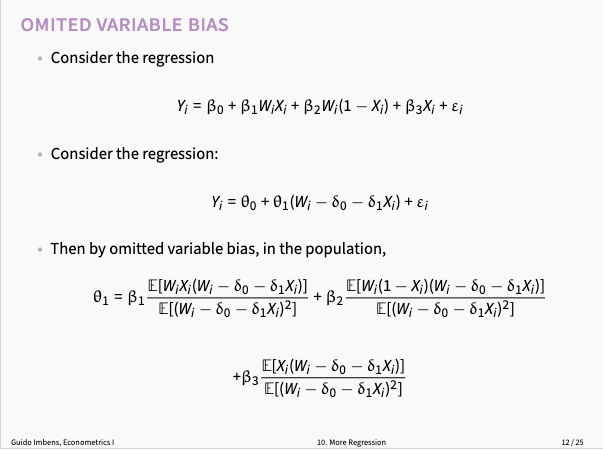
\includegraphics[width=0.7\textwidth]{images/wk7-1.png}
    \caption{p.12 of the slides}
    \label{fig:ovb_logic}
\end{figure}

Figure \ref{fig:ovb_logic} shows the slides 11.12. In this figure we derived the relationship between the parameters of two regression models, using the so-called OVB logic.
The way I understood the logic is that, we start with the first regression model and consider that the true DGP.
In the second regression, we have the variable $W_i - \delta_0 - \delta_1 X_i$ as the univariate regressor.
Denote this regressor by $Z_i$.
We can decompose the correlation between this variable and the outcome $Y_i$ into three parts, or channels:

\begin{itemize}
    \item the channel of $W_iX_i$: computed by the product of the direct effect of $W_iX_i$ on $Y_i$, which is $\beta_1$, and the correlation between $W_iX_i$ and $Z_i$, which is the cross-moment in the slide.
    \item the channel of $W_i(1-X_i)$: computed by the product of the direct effect of $W_i(1-X_i)$ on $Y_i$, which is $\beta_2$, and the correlation between $W_i(1-X_i)$ and $Z_i$, which is the cross-moment in the slide.
    \item the channel of $X_i$: computed by the product of the direct effect of $X_i$ on $Y_i$, which is $\beta_3$, and the correlation between $X_i$ and $Z_i$, which is the cross-moment in the slide.
\end{itemize}

This kind of logic helped me ``memorize'' the OVB logic and the formula; however, I still don't understand how equation in the slide makes sense.
This doesn't look like the FWL theorem to me, because in that case, we were comparing two regression models where one has the entire set of covariates, and the other has some omitted variables.
That doesn't directly translate to the equations I see in the slide.

\section{Slides 13 Lasso Regression}

This question relates to the figure comparing the coefficients of the lasso and the ridge regression:

\begin{figure}[h]
    \centering
    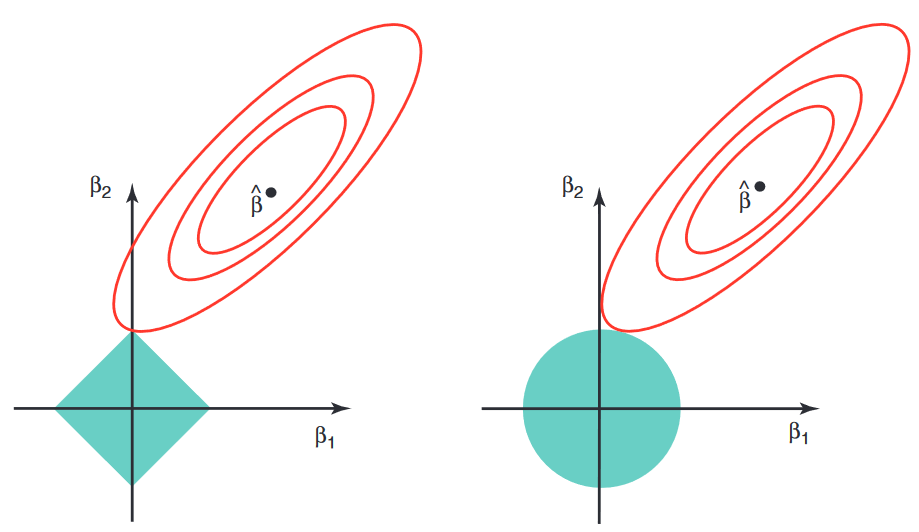
\includegraphics[width=0.7\textwidth]{images/wk7-2.png}
    \caption{LASSO vs. Ridge Regression}
    \label{fig:lasso_ridge_comparison}
\end{figure}

I'm more interested in the shape of the ovals. The oval here looks like it's stretched along the $y=x+k$ line, but Guido drew an oval stretched along the $y=-x+k$ line (sort of stretched from NW to SE) when we have multicollinear variables.
I wonder how to understand the shape of the ovals. 
{\color{blue} As an update from Nov 12, I asked this question to Guido, but I didn't fully understand his answer yet. He said that the oval becomes a circle if the covariates are fully independent, 
but becomes more oval if we have collinearity. 
But my question is more related to `which' direction the oval would be strectched to.
}

One intuition I had about these figures before was comparing them to the utility curve and the budget constraint in the consumer theory – that way, I could kind of think of the ovals as the indifference curves.
I wonder if we can apply a similar intuition and compare the collinear case to the perfect substitute case in consumer theory – we have a flatter tangent of the oval(indifference curve) when we have substitutable variables(goods).

\section{Slides 14 Clustering}

\begin{figure}[h]
    \centering
    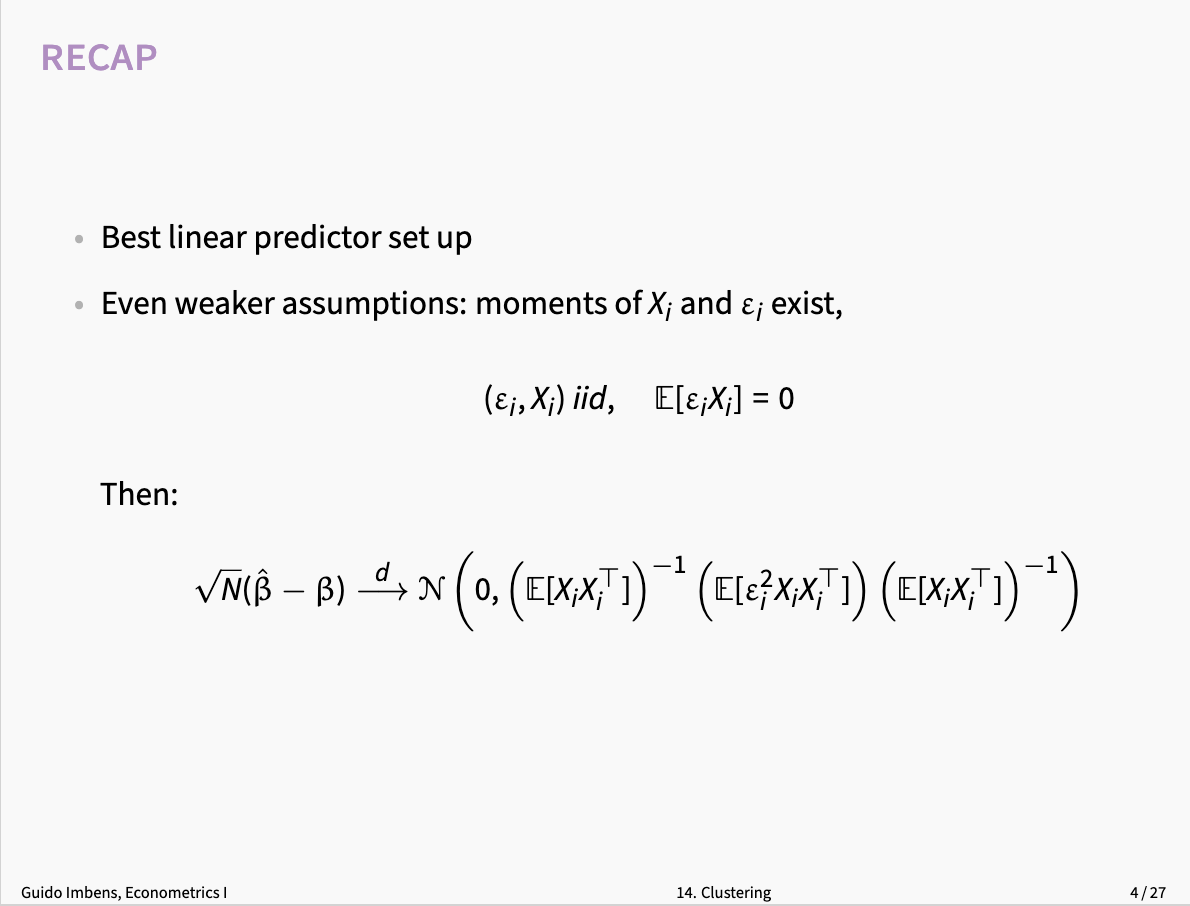
\includegraphics[width=0.7\textwidth]{images/wk7-3.png}
    \caption{Clustering}
    \label{fig:clustering}
\end{figure}

In the slide above(fig. \ref{fig:clustering}), it assumes that the error term and the covariates are iid distributed.
Is this a typo? 
To write the true asymptotic variance in the way it is written down on the slide,
isn't `independence' sufficient for this case, and the error terms need not have the exact same distribution?

\end{document}
